\documentclass[11pt, fleqn]{article}

\usepackage[usenames,dvipsnames,svgnames,table]{xcolor}
\usepackage{amsmath}
\usepackage{amsfonts}
\usepackage[margin=1in]{geometry} % To set the margin widths
\usepackage{graphicx}
\usepackage{listings}
\usepackage{multirow}
\usepackage{tabularx}
\usepackage{varioref}
\usepackage[noabbrev,capitalize]{cleveref}
\usepackage[group-separator={,}]{siunitx}
\usepackage{subcaption}
\usepackage{titlesec}
\usepackage{lscape}
\usepackage{bm}
\usepackage[titletoc,toc,title]{appendix}

\lstset{
  frame=single,
  basicstyle=\ttfamily,% print whole listing small
  language=R,
  aboveskip=3mm,
  belowskip=3mm,
  showstringspaces=false,
  columns=flexible,
  numbers=none,
  commentstyle=\color{ForestGreen},
  stringstyle=\color{Maroon},
  breaklines=true,
  breakatwhitespace=true,
  tabsize=2,
  literate={<-}{{$\gets$}}1 {~}{{$\sim$}}1
}

\sisetup{output-exponent-marker=\textsc{e}}

\setlength{\parskip}{12pt} % Sets a blank line in between paragraphs
\setlength\parindent{0pt} % Sets the indent for each paragraph to zero

\begin{document}

\title{Machine Learning (41204-01)\\HW \#7}
\author{Will Clark and Matthew DeLio \\
\textsf{\{will.clark,mdelio\}@chicagobooth.edu} \\
University of Chicago Booth School of Business}
\date{\today}
\maketitle

\section{Zachary's Karate Club}

\begin{figure}[!htb]
\centering
\caption{Zachary's Karate Club and Factions}
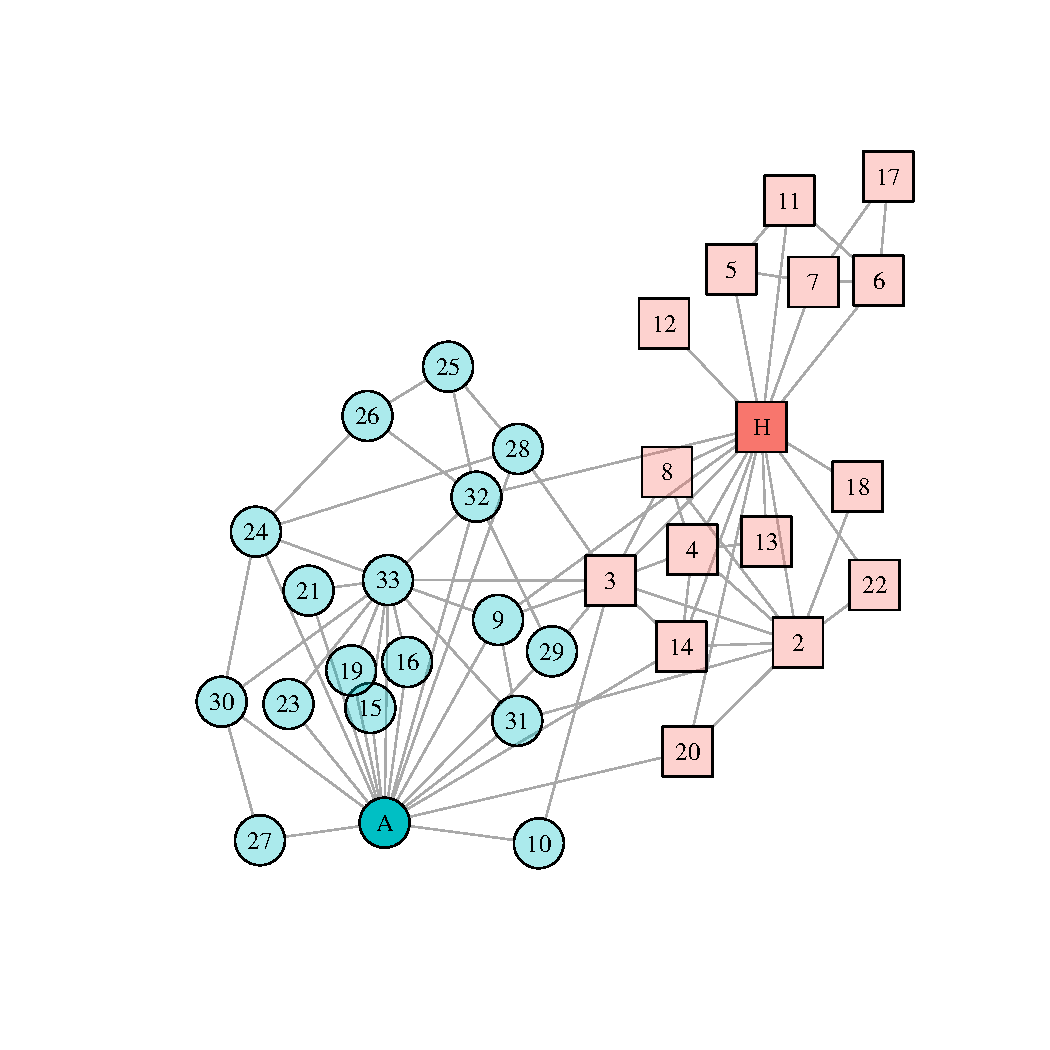
\includegraphics[scale=.5,trim={0.75in 0.75in 0.75in 0.75in}, clip=True]{karate_network.pdf}
\label{fig:karate_network}
\end{figure}

We used the following algorithms to try and determine the underlying community structure in Zachary's karate club. The results are visualized in \cref{fig:edge_betweenness}-\cref{fig:walktrap}.
\begin{itemize}
\item \textbf{Edge Betweenness}: A hierarchical algorithm that we cut to obtain two groups. The default setting is for the algorithm to consider the network edge weights, but in doing so the algorithm misclassifies two vertices (Actors 3 and 14; see \cref{fig:edge_betweenness}). By ignoring the edge weights, the algorithm only mis-classifies one vertex (Actor 3). 
\item \textbf{Greedy Modularity Optimization (Fast Greedy)}: A hierarchical algorithm that we cut to obtain two groups. It correctly predicts the faction for all vertices (see \cref{fig:fast_greedy}).
\item \textbf{Infomap}: A non-hierarchical algorithm that splits the data into 3 groups. Two groups are made entirely of members from Mr. Hi's faction, so there are no mis-classifications.
\item \textbf{Propagating Labels}: A non-hierarchical algorithm that splits the data into 3 groups. Two groups are made entirely of members from Mr. Hi's faction, so there are no mis-classifications. 
\item \textbf{Leading Eigenvector}: A hierarchical algorithm that we cut to obtain two groups. ???? WHAT'S THE DEAL?
\item \textbf{Multi-level Modularity Optimization (Louvain)}: A non-hierarchical algorithm that splits the data into X groups.
\item \textbf{Optimal Structure}: A non-hierarchical algorithm that splits the data into X groups.
\item \textbf{Statistical Mechanics (Spinglass)}: A non-hierarchical algorithm that splits the data into X groups.
\item \textbf{Short Random Walks (Walktrap)}: A hierarchical algorithm that we cut to obtain two groups. It correctly predicts the faction for all vertices.
\end{itemize}

%%%%%%%%%%%%%%%%%%%% KARATE COMMUNITY GRAPHS %%%%%%%%%%%%%%%%%%%%
\begin{figure}
\centering
\begin{subfigure}[b]{0.32\textwidth}
\caption{Edge Betweenness}
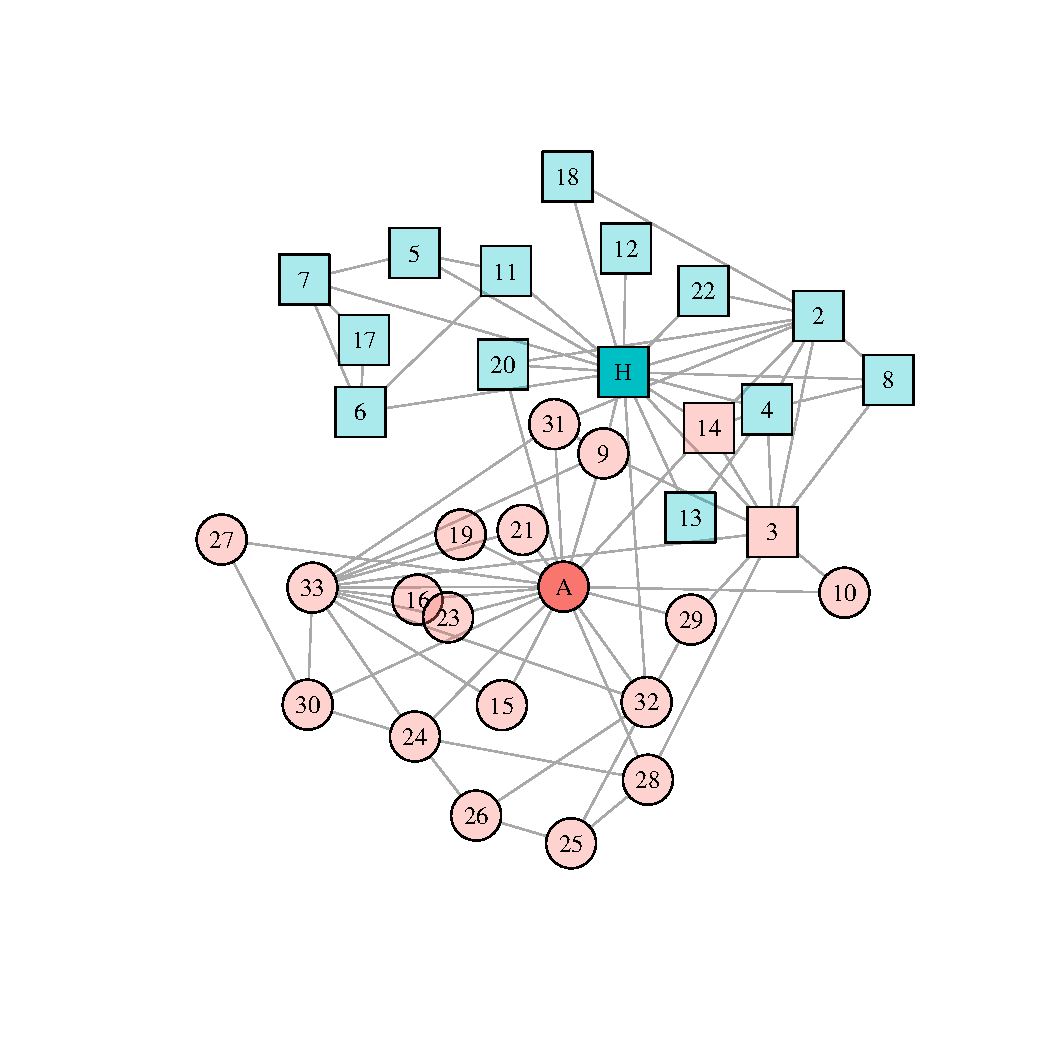
\includegraphics[width=\textwidth,trim={0.75in 0.75in 0.75in 0.75in}, clip=True]{edge_betweenness.pdf}
\label{fig:edge_betweenness}
\end{subfigure}
\hfill
\begin{subfigure}[b]{0.32\textwidth}
\caption{Greedy Modularity \\Optimization}
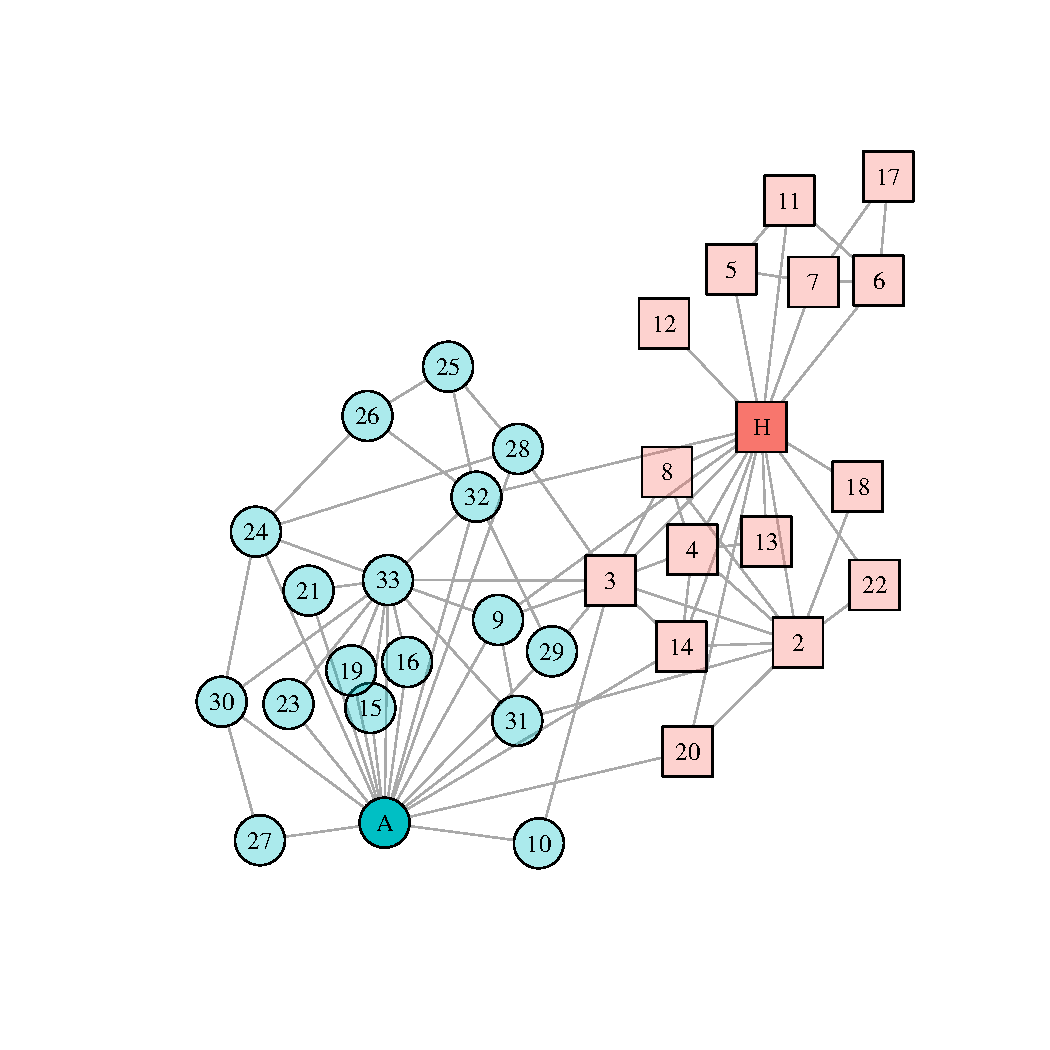
\includegraphics[width=\textwidth,trim={0.75in 0.75in 0.75in 0.75in}, clip=True]{fast_greedy.pdf}
\label{fig:fast_greedy}
\end{subfigure}
\hfill
\begin{subfigure}[b]{0.32\textwidth}
\caption{Infomap}
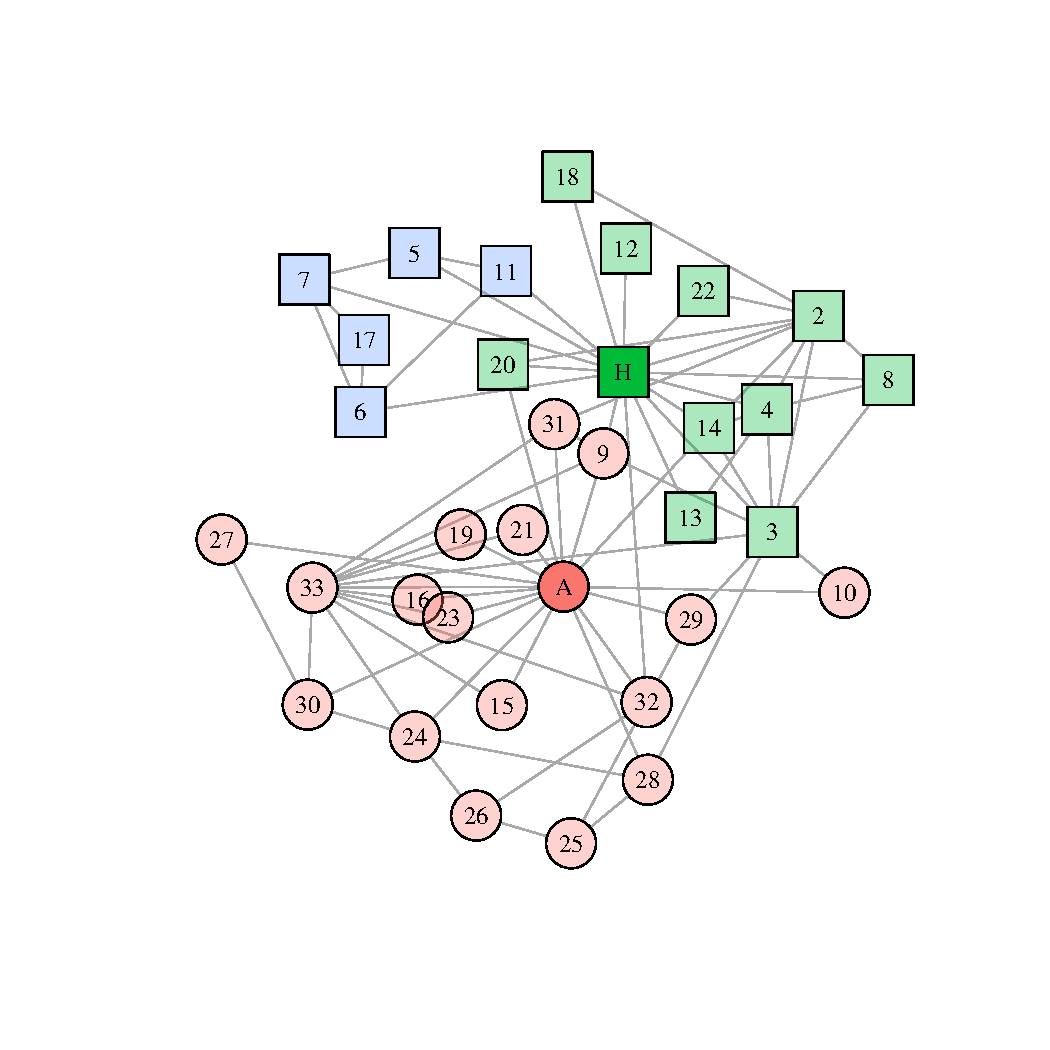
\includegraphics[width=\textwidth,trim={0.75in 0.75in 0.75in 0.75in}, clip=True]{infomap.pdf}
\label{fig:infomap}
\end{subfigure}

\begin{subfigure}[b]{0.32\textwidth}
\caption{Propagating Labels}
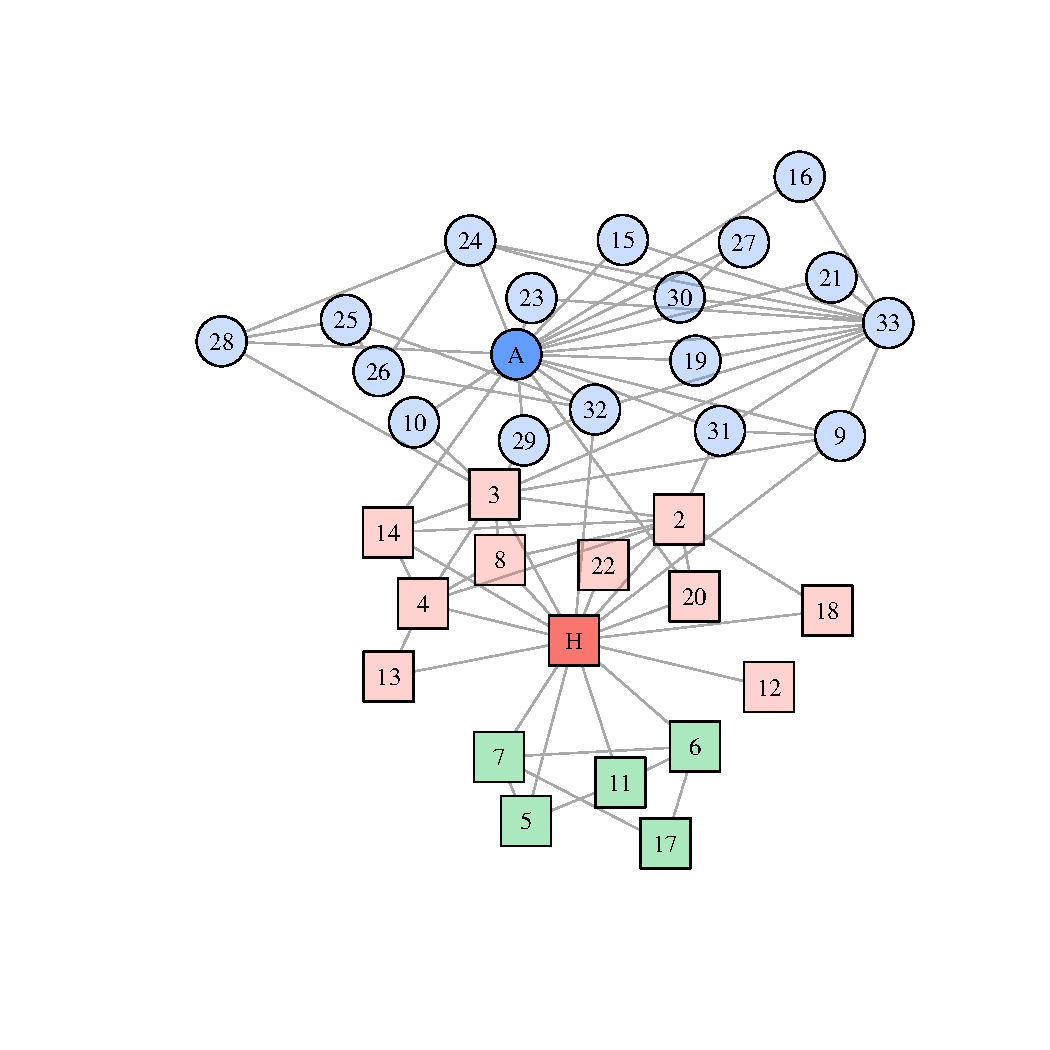
\includegraphics[width=\textwidth,trim={0.75in 0.75in 0.75in 0.75in}, clip=True]{label_prop.pdf}
\label{fig:label_prop}
\end{subfigure}
\hfill
\begin{subfigure}[b]{0.32\textwidth}
\caption{Leading Eigenvector}
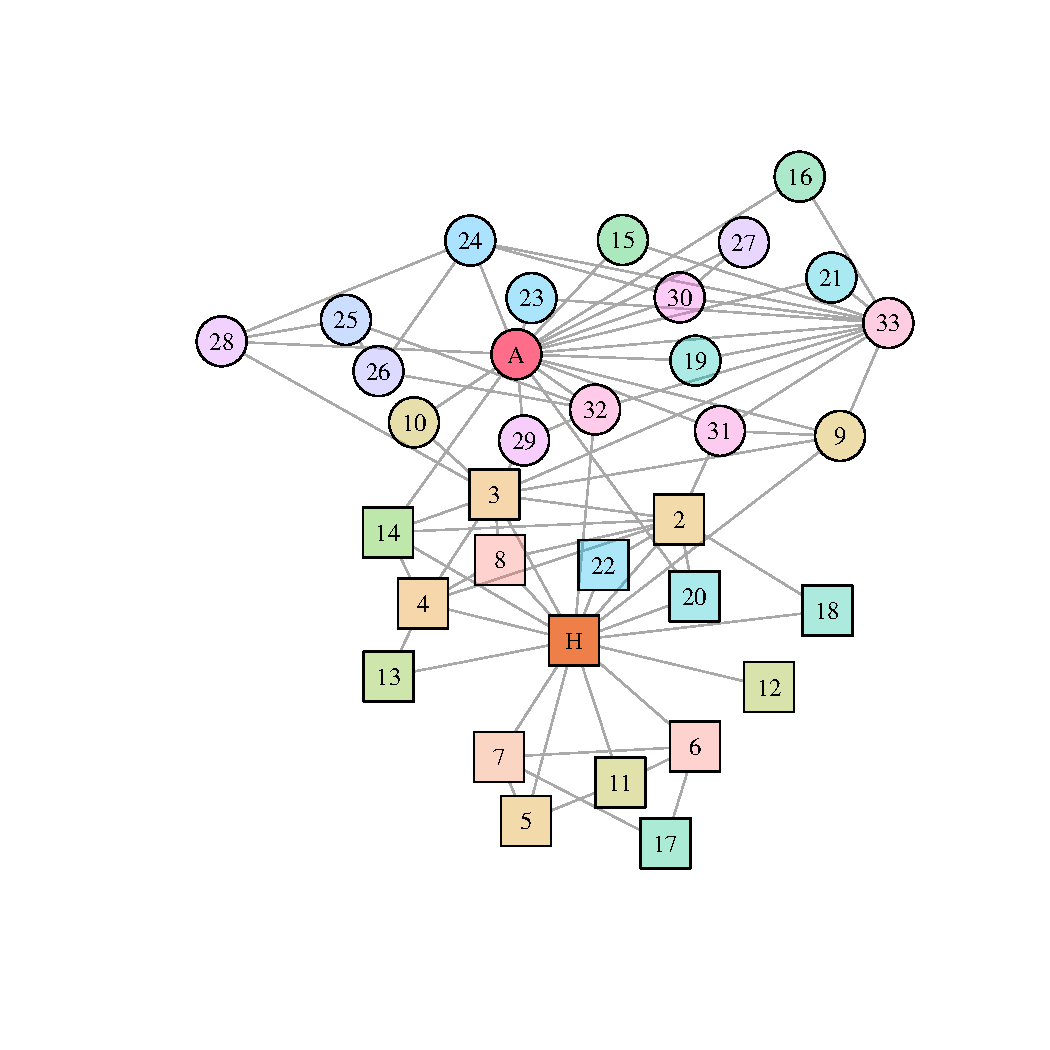
\includegraphics[width=\textwidth,trim={0.75in 0.75in 0.75in 0.75in}, clip=True]{leading_eigen.pdf}
\label{fig:leading_eigen}
\end{subfigure}
\hfill
\begin{subfigure}[b]{0.32\textwidth}
\caption{Multi-level Modularity \\Optimization}
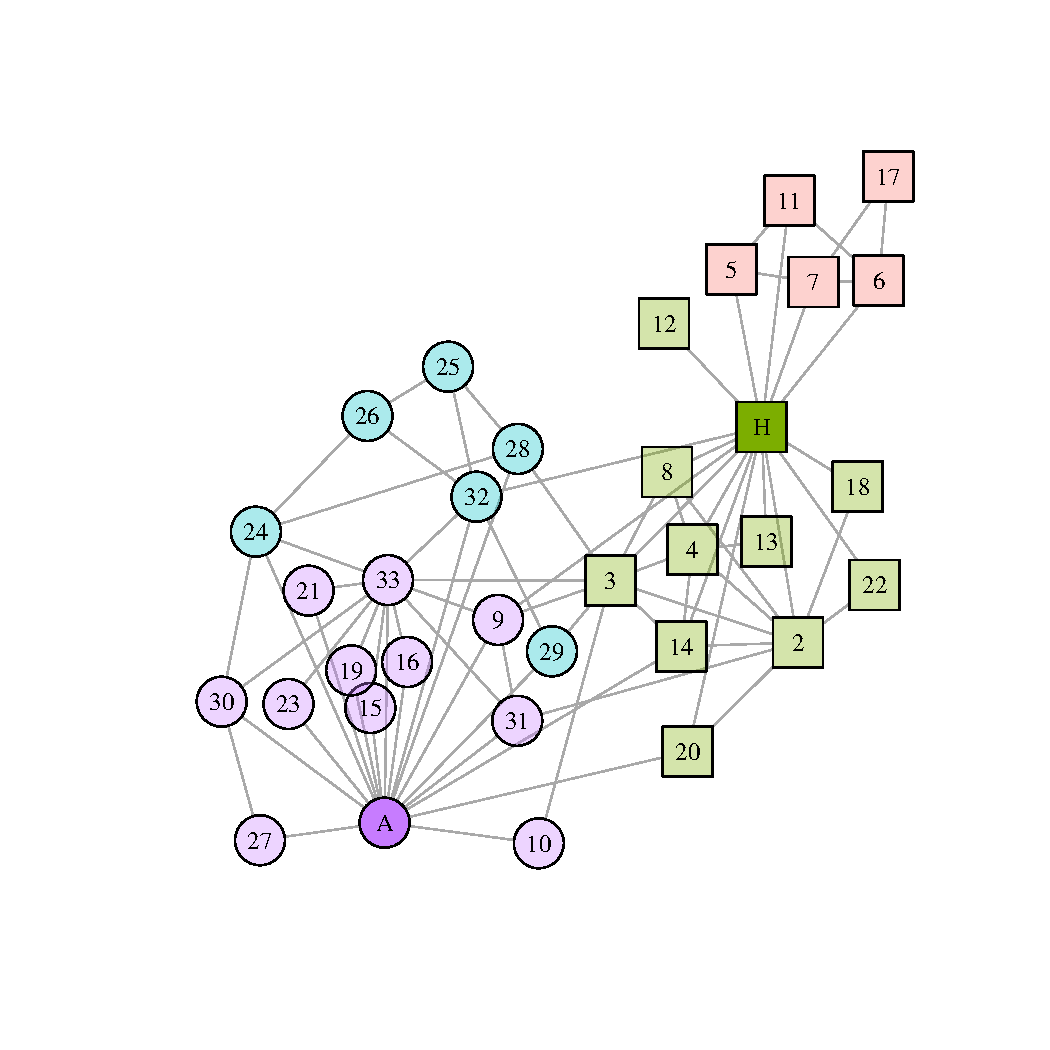
\includegraphics[width=\textwidth,trim={0.75in 0.75in 0.75in 0.75in}, clip=True]{louvain.pdf}
\label{fig:louvain}
\end{subfigure}

\begin{subfigure}[b]{0.32\textwidth}
\caption{Optimal Structure}
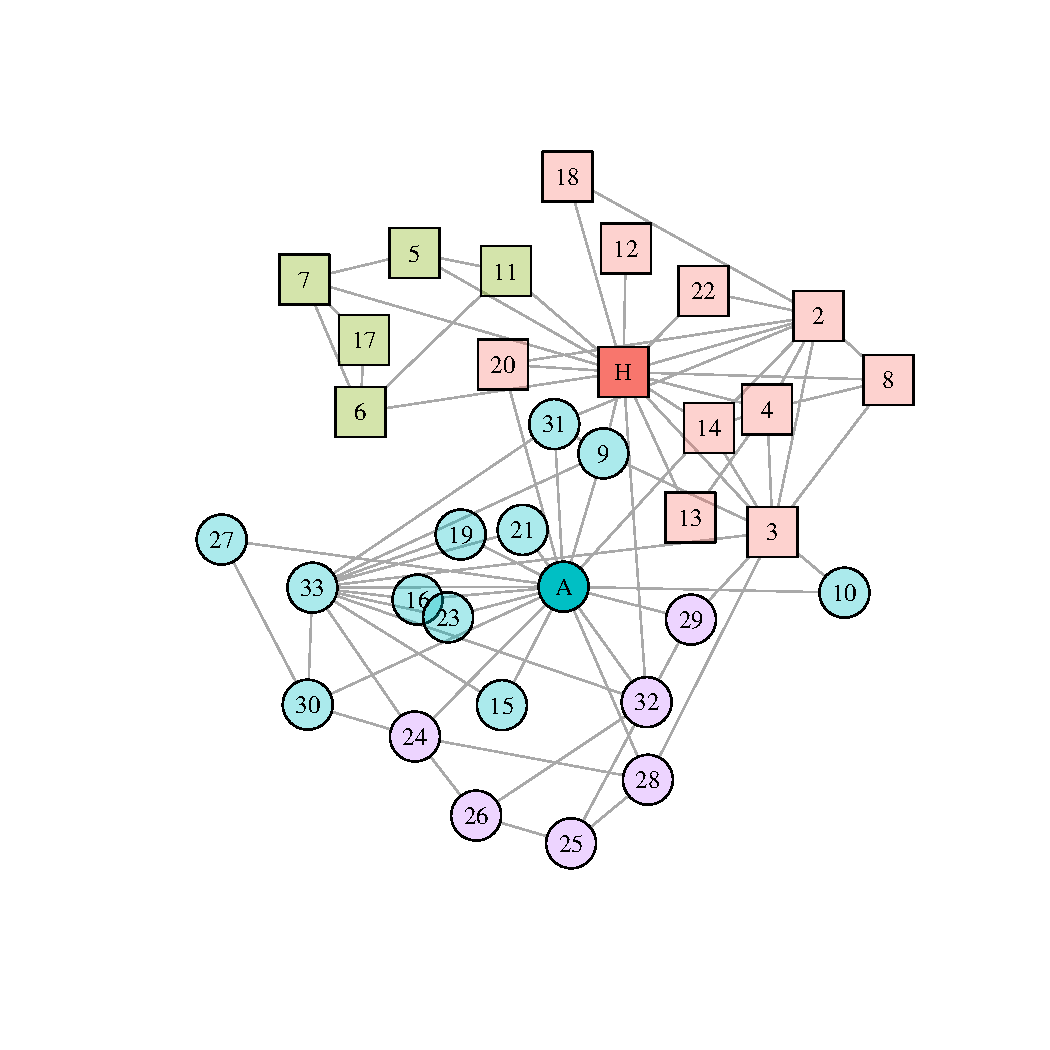
\includegraphics[width=\textwidth,trim={0.75in 0.75in 0.75in 0.75in}, clip=True]{optimal.pdf}
\label{fig:optimal}
\end{subfigure}
\hfill
\begin{subfigure}[b]{0.32\textwidth}
\caption{Statistical Mechanics}
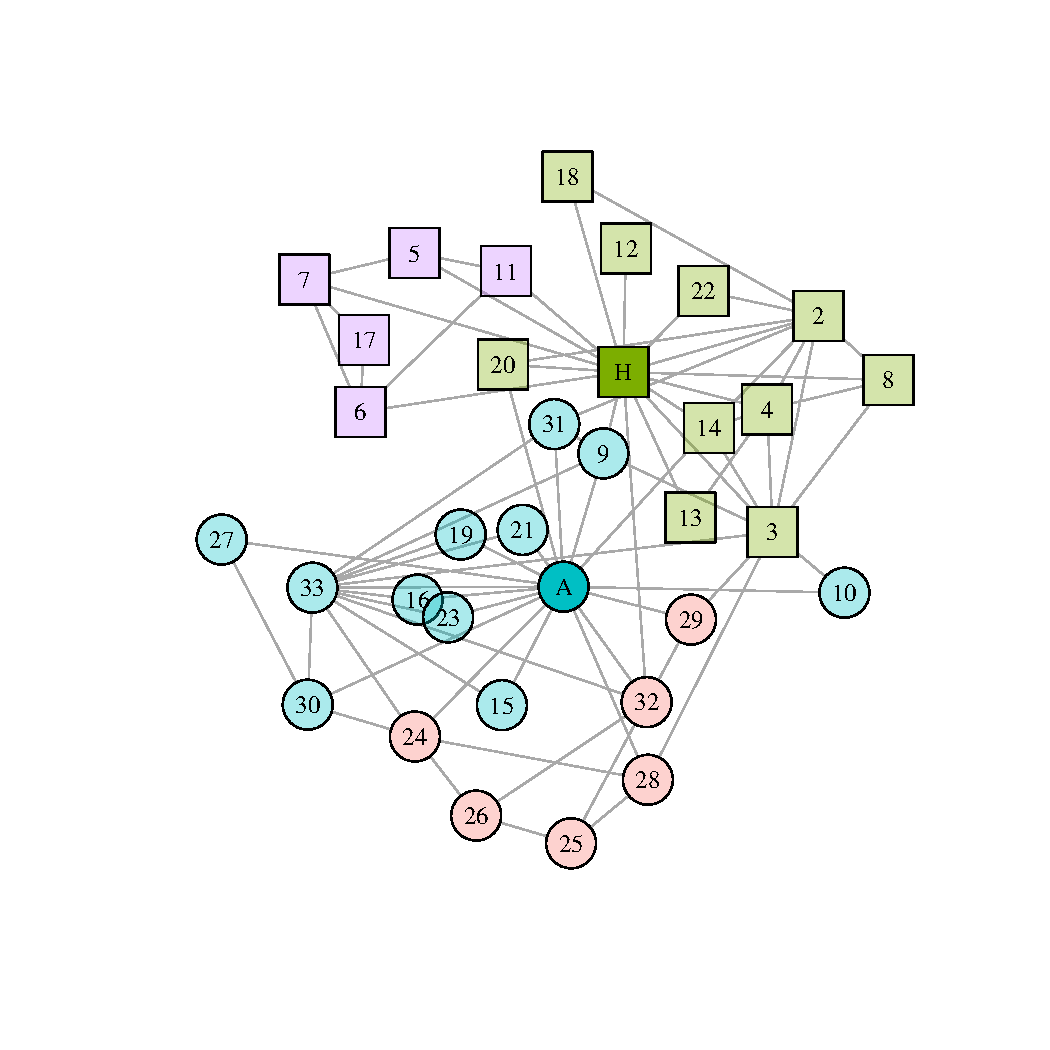
\includegraphics[width=\textwidth,trim={0.75in 0.75in 0.75in 0.75in}, clip=True]{spinglass.pdf}
\label{fig:spinglass}
\end{subfigure}
\hfill
\begin{subfigure}[b]{0.32\textwidth}
\caption{Short Random Walks}
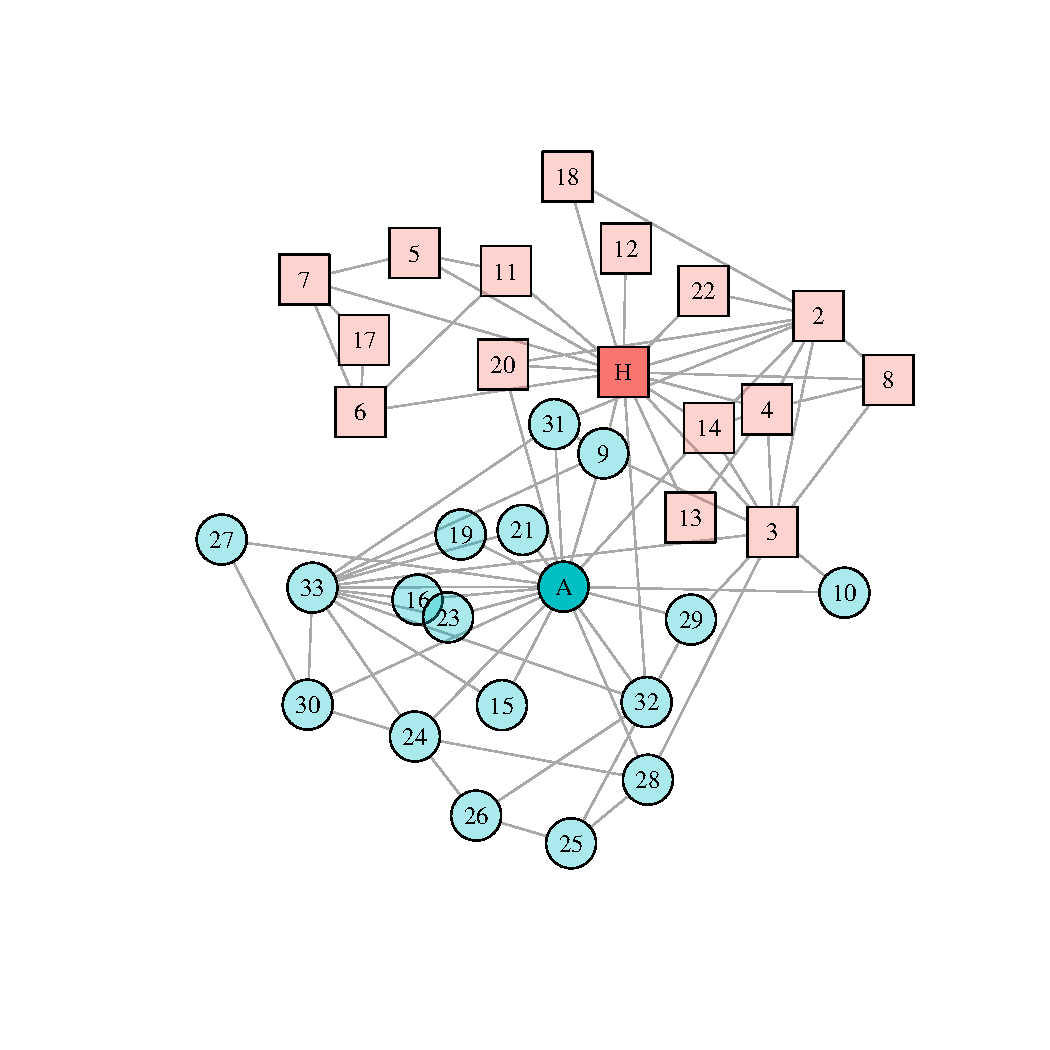
\includegraphics[width=\textwidth,trim={0.75in 0.75in 0.75in 0.75in}, clip=True]{walktrap.pdf}
\label{fig:walktrap}
\end{subfigure}
\caption{Community Detection Algorithms for Zachary's Karate Club}
\end{figure}
%%%%%%%%%%%%%%%%%%%%%%%%%%%%%%%%%%%%%%%%%%%%%%%%%%%%%%%%%%%%%%%%%

\section{Wikipedia}

\begin{appendices}

\end{appendices}

\end{document}

% \input{.tex}

% \begin{figure}
%   \centering
%   \begin{subfigure}[b]{0.49\textwidth}
%     \caption{}
%     \includegraphics[width=\textwidth]{.pdf}
%     \label{fig:}
%   \end{subfigure}
%   \hfill
%   \begin{subfigure}[b]{0.49\textwidth}
%     \caption{}
%     \includegraphics[width=\textwidth]{.pdf}
%     \label{fig:}
%   \end{subfigure}
%   \caption{}
% \end{figure}

% \begin{figure}[!htb]
%   \centering
%   \caption{}
%   \includegraphics[scale=.5]{.pdf}
%   \label{fig:}
% \end{figure}

